\chapter{Resultater}

Der er i dette projekt udarbejdet en prototype, som kan undersøge muligheden for en automatiseret metode at isolerer langerhanske øer. Der er udviklet et færdig system, som har potentiale til at isolere langerhanske øer, det vil sige at produktet kan isolere plantefrø, som er brugt i en simuleringsvæske. Derfor er de mekaniske og elektriske dele på plads, til videre undersøgelser af konceptet. I projektet er der også opnået en billedebehandling der understøtter konceptet, i kraft af hastigheden af processeringen af de simuleret billeder. Der er brugt simulerede billeder, fordi det indkøbte kamera ikke har været af tilstrækkelig kvalitet. fxnote{den kan ikke sorter plantefrø endnu!}

\section{Det udviklede system}
Det udviklede system til isolering af langerhanske øer består af et software program udviklet i Matlab og en række hardware komponenter som styres vha. en Arduino.


 
\subsection{Brugergrænseflade} 
Software delen består af en brugergrænseflade, hvor operatøren har mulighed for at interagere med systemet. Figur \ref{fig:finalgui} viser hvordan brugergrænsefladen er opbygget. Operatøren har via en knap mulighed for at starte og stoppe sorteringscyklussen. En række tekstfelter med feedback,  giver operatøren information om den igangværende sorteringscyklus, herunder antal sorterede øer, indholdet tilbage i opløsningsbeholderen og status for systemet. Et kamera feed er herudover vist, som giver operatøren mulighed for at følge indholdet, der løber igennem slangen. Under kamera feedet vises et behandlet billede af feedet fra kameraet. Hvis en ø er detekteret markeres den på begge feeds med en grøn cirkel.

 \begin{figure}[H]
	\centering
	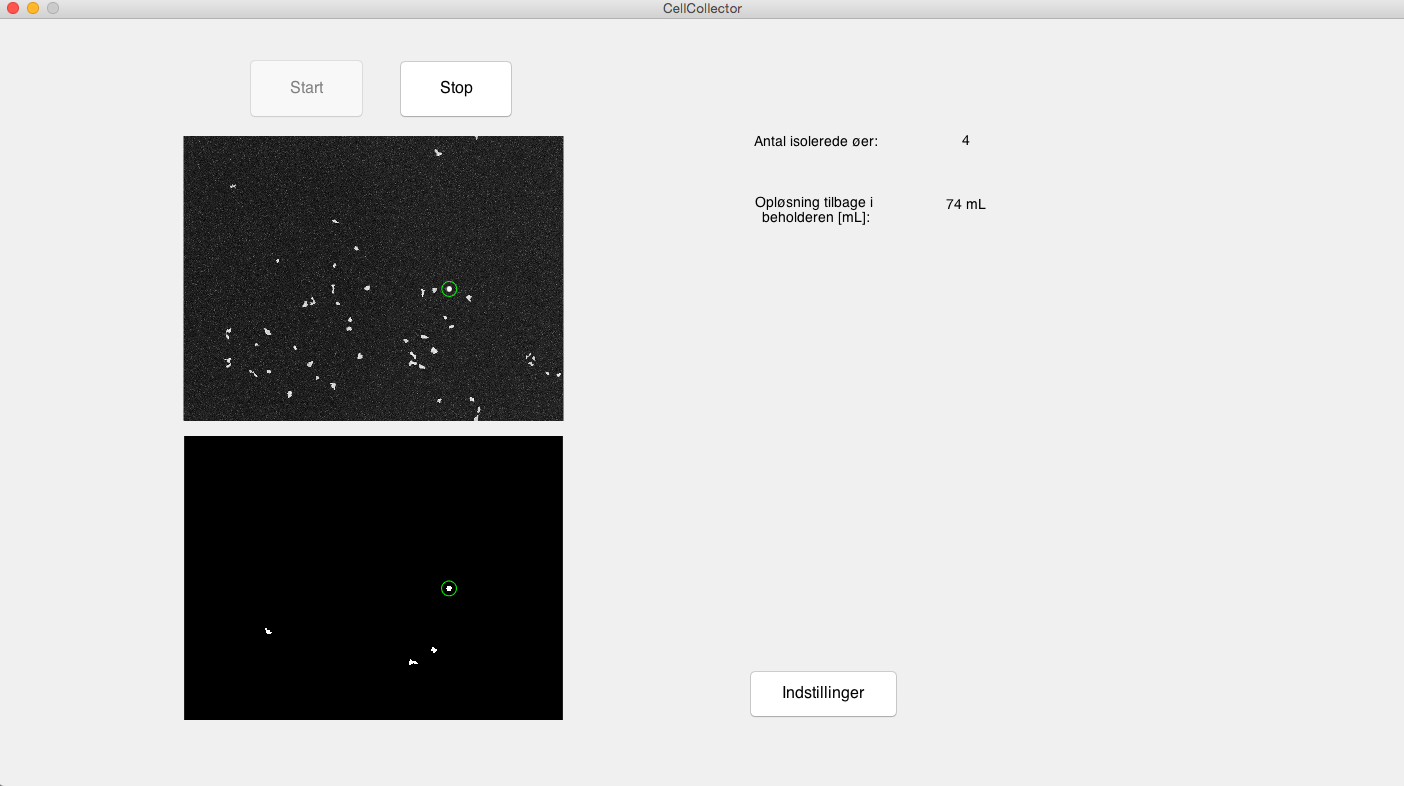
\includegraphics[width=1\textwidth]{billeder/gui_main.png}
	\caption{Brugergrænsefladen på prototypen}
	\label{fig:finalgui}
\end{figure}

\subsection{Hardwaren}

Den overordnet funktion af hardwaren er, at pumpe opløsningsvæsken forbi kameraet hen forbi ventilen til \textit{wastebeholderen} eller beholderen til de isoleret langerhanske øer. For at fremvise projektets færdige resultater, er kredsløbet og layoutet til det udarbejdede printkort til produktet indsat her under på figur XX. Til et overordnet overblik over hardwaren i projektet henvises der til figur \ref{fig:bdd_Hardware}. Printkortet er lavet som et shield til \textit{Arduino} udviklingskortet. Shieldet kan sættes direkte oven på arduinoen, på printkortet er der stik til at forsyne og videregive signaler til hardware komponenterne. Komponenterne er pumpen, der skaber flowet i slangen, ventilen som isolerer øerne, kameralyset lyser øerne op så kameraet bedre kan detektere dem. Derudover er vægtcellen også forsynet i gennem printet. Printkortets layout er udarbejdet i \textit{Eagle}, hvor lagene er eksporteret til \textit{gerber} filer. Filerne er sendt til printfremstilling ved Ingeniørhøjskolens værksted.

\subsubsection{Det samlede kredsløb}

Kredsløbet for det samlede print er indsat her nedenfor, kredsløbet beskriver hvordan delene er forbundet. \fxnote{beskriv nærmere nær printet er lavet}
Se diagrammet for printet på figur XX

\subsubsection{Det færdig print layout}
Nedenfor på figur XX kan layoutet ses i \textit{Eagle}. På printet er der to integrerede kredsløb, den ene(IC1) er en L293D som bla. bliver brugt som motordriver i projektet. Motordriveren forsynes eksternt og bruger igennem denne til at forsyne motor, kameralys og ventil. Kort fortalt tager motordriveren signalet fra arduinoen og efterligner det, men i stedet leverer effekten i gennem den eksterne forsyning. Det andet(IC2) integrerede kredsløb består af en operationsforstærker, som primært har til opgave at forstærke outputtet fra vægtcellen til arduinoens analog-digital konverter(ADC). Det gøres fordi outputtet fra vægtcellen er i mV og arduinoens ADC har en arbejdsspænding på 0V til 5V.  

\subsection{Ikke-elektroniske dele}
De ikke-elektroniske dele, består af beholdere, slanger og adaptere. I projektet er der fokuseret på opløsningsbeholderen, hvor der er indkøbt en 250ml beholder med et specielt låg. Igennem låget går en teflonslange, for at tætne denne tilslutning er der en forskruning som både aflaster og tætner i låget. I låget er der også et luftfilter, som forhindre støv og andre små partikler for at komme ned i opløsningen. Filteret skal være der for at undgå dannelse af undertryk i beholder, når pumpen suger opløsningsvæsken igennem systemet. Da teflonslangen ikke er eftergivende, er der brugt silikoneslanger til stykket igennem pumpen og resten af systemet. Fordi teflonslangen er for hård til, at pumpen kan sammenpresse den og derved skabe flow i opløsningen. For at kunne gå fra teflonslangen til silikoneslangen er der brugt en adapter. Se styklisten mm. i projektdokumentation afsnit XX.
\fxnote{illustration af de ikke-elektroniske dele gælder også i dokumentationen}

%\subsubsection{Styreenheden} 
%Til at kontroller hardware komponenterne i systemet er der brugt en styreenhed i form af et arduino udviklingsboard, som er velegnet til producering af prototyper som i dette projekt. Udover at styre komponenterne sikre arduinoen også integrationen, mellem computeren og hardwaren. Derfor er det styreenheden der kontroller flow hastigheden, styrken af kameralyset samt åbning og lukning af ventilen. Se afsnit XX i projektdokumentationen for uddybende dokumentation for design og implementering af styreenheden.

%\subsubsection{Motordriveren}
%Motordriveren bruges i systemet til at forsyne pumpen, ventil og kameralyset. Motordriveren er nødvendig da Arduinoen ikke kan trække strøm nok til, at trække de nævnte komponenter. Motordriveren består af en L293D\fxnote{er det for specifikt?}, som efterligner signalerne modtaget af arduinoen og videre giver dem til komponenterne, men med forsyning igennem en strømforsyning der i modsætning til arduinoen kan levere den nødvendige strøm. Ved PWM signalet hæver motordriveren amplituden, med strømforsyningensspænding i stedet for arduinoensspænding. Se afsnit XX i projektdokumentationen for uddybende dokumentation for design og implementering af motordriveren.

%\subsubsection{Ventil}
%Ventilen skal kort sagt isolere de langerhanske øer, når kameraet har detekteret en ø. For at være sikker på at isoleringen er succesfuld er der implementeret en tidsforsinkelse på ventil når den er åben. Denne tid er en prioritering for det er uønsket, at få rest vævet med i den isoleret ø beholder. Tiden er i projektet beregnet og senere estimeret ud fra forsøg med simuleringsvæsken. Se afsnit XX i projektdokumentationen for uddybende dokumentation for design og implementering af ventilen.

%\subsubsection{Pumpe}
%Pumpens opgave er at skabe et flow i slanger og der ved drive opløsningsvæsken forbi kameraet og hen til ventilen. I projektet er der brugt en peristaltisk pumpe, der skaber et flow ved at sammenpresse slangen ved rotation. Denne pumpe type skaber et stabilt flow med mulighed for variable hastighed, ved hjælp af PWM forsyning fra arduinoen igennem motordriveren. Se afsnit XX i projektdokumentationen for uddybende dokumentation for design og implementering af pumpen.

%\subsubsection{Vægtcellen}
%Vægtcellen vejer opløsningsbeholderen og stopper systemet når der ikke er mere væske i beholderen. Vægtcellens output er i millivolt hvilket har medført at det skulle forstærkes, for at ADCens opløsning på arduionen kunne udnyttes fuldt ud. Derfor er der brugt en operationsforstærker til dette formål. Yderligere er vægtcellen kalibreret i softwaren ved hjælp af lineær regression. Der kan læses mere omkring implementeringen af vægtcellen i afsnit XX for design og implementering af komponenten, både for software og hardware.

%\subsubsection{Kameralyset}
%I prototypen er der brugt fire lysdioder til, at have fuldstændig kontrol over lyset til kameraet. Det er erfaret igennem enhedstest af kameraet, at lyset som påvirker kameraet er meget vigtig for detektionen af øerne. Se afsnit XX i projektdokumentationen for yderligere dokumentation af kameralyset.

 \section{Ventil tidsinterval}
Tidsintervallet mellem kameraet og ventilen er en vigtig faktor i systemet. Fordi intervallet beskriver tiden fra, at kameraet har detekteret en ø til den er kommet hen til ventilen, hvor den skal isoleres. En estimation er beregnet igennem nedenstående formler. Kravet fra kunden hedder 30 øer i minuttet, derfor skal systemet som minimum have en flow hastighed på 11,25 ml/min. Se formel \ref{eg:ohastighed} for udregningen.

\begin{align}
\frac{\text{Opløsningsstørrelse}}{\text{Antal øer i opløsning}} = \frac{\SI{150}{\milli\liter}}{400\text{ øer}}*30 = \SI{11,25}{\milli\liter/minut} 
\label{eg:ohastighed}
\end{align}(\textit{jf. Søren Gregersen})

For at sorteringen af langerhanske øer er succesfuld, kræver det en beregning af den tid det tager for en langerhansk ø, at komme fra kameraet til ventilen. Det kan estimeres ud fra det volumenet af slangen, i mellem kameraet og ventil \ref{eg:slangevolume}.

\begin{align}
V=\pi*r^2*h=\pi*\frac{\SI{51}{\micro\metre}}{2}*\SI{5}{\centi\metre}=\SI{0,04}{\milli\liter}
\label{eg:slangevolume}
\end{align}

 Det vil sige at med et flow på $\SI{11,25}{\milli\liter/minut}$, som er beregnet ud fra formlen \ref{eg:ohastighed}. Der ud fra kan tiden fra kamera til ventil beregnes ved formelen \ref{eq:tidsintervallet}. 
 
\begin{align}
\frac{\SI{11,25}{\milli\liter/minut}}{\SI{60}{\second}}=\SI{0,1875}{\milli\liter/s}\to\frac{\SI{0,04}{\milli\liter}}{\SI{0,1875}{\milli\liter/s}}=\SI{0.213}{\second}
\label{eq:tidsintervallet}
\end{align} 

i følge bilag \ref{bilag:ventil} har ventilen et volumen $\SI{27}{\micro\liter}$

\begin{align}
\text{Tid for udtømning af ventilen} = \frac{\text{ventil volume}}{\text{ml pr. sekund}}=\frac{\SI{27}{\micro\liter}}{\SI{0,1875}{\milli\liter/s}}=144ms
\label{eq:ventilvolume}
\end{align}

Fra de overstående beregninger kan det observeres, at tidsintervallet mellem kamera og ventilen er 213 millisekunder. Ud fra dette tidsinterval skal systemets tid fra, at kameraet har detekteret en ø til at ventilen kan åbne trækkes fra. Ligeledes skal ventilens lukketid også trækkes fra. I følge bilag \ref{bilag:ventil} har ventilen en åbningstid op til 20ms og en lukketid på op til 30ms. Til denne tid skal der yderligere tillægges tiden for kommunikation fra computer til arduino.
\begin{align}
Timerdelay=213ms-40ms-50ms=123ms
\label{eq:timerdelay}
\end{align} 
\fxnote{tiderne skal testes i en integrationstest}

Dette er tiden der skal gå fra kameraet har detekteret en ø, til den samme ø er ved ventilen. Der er implementeret et timer delay til dette i softwaren. For at være sikker på at øen bliver isoleret, er der implementeret endnu et timer delay der beskriver åbningstiden for ventilen. Til dette skal ventilen åbne lidt før og lukke lidt efter. Derfor bør tidsintervallet mellem kamera og ventil differentieres med 20ms og 20ms efter. I formel \ref{eq:ventilvolume} skal der bruges 144ms for at tømme ventilens volume, derfor er timerdelayet til åbningstiden for ventilen på 184ms. 
Åbningstiden er et kompromis, fordi det ikke er favorable at det eksokrine væv kommer over i den isoleret beholder, men samtidigt skal sandsynligheden for at ventilen er åben når øen kommer være så høj som mulig.

\newpage
\section{Kamera}
Det indkøbte kamera viste sig ikke at være  tilstrækkelig kvalitet i gennem en enhedstest. Der kunne ikke skelnes mellem det eksokrine væv og de langerhanske øer. Yderligere blev det erfaret at lyset er utrolig vigtigt, derfor er ideen med kamerahuset en nødvendighed for at kontroller lyset til kameraet. Der kan læses mere om enhedstesten af kameraet i afsnit XX \fxnote{Indsæt nummer} i projektdokumentationen. Til at erstatte kameraet blev der i stedet genereret en række billeder, som skulle simulere flowet af opløsningsvæske i gennem slangen.

\subsection{Kamerasimulation}
Til at generere et billedsæt, der simulerer langerhanske øer, er der udviklet et Matlab script. Billederne der er valgt stammer fra det indkøbte kamera. Grunden til de kan anvendes som grundlag for genereringen af billeder, på trods af kameraets utilstrækkelige kvalitet, er at øerne og det ekstra væv er adskilt i de enkelte billeder. Dette muliggør en seperat segmentering af øer og væv, som  herefter kan sammensættes til billeder der ligger tæt op af det man observerer gennem et almindeligt mikroskop. 

Flowsimuleringen er opbygget på den måde, at den består af henholdvis en sekvens indeholdende en langerhansk ø efterfulgt af en sekvens uden en ø. I selve programmet indlæses et nyt billede hvert 0,1 sekund. Derfor skal der generes en passende mængde billeder, som programmet kan indlæse. Simuleringen er implementeret så der minimum genereres 252 eller maksimalt 432 billeder, hvilket giver en samlet sekvenslængde på 25,2 eller 43,2 sekund. Grunden til at antallet af billeder varierer er at længden af sekvensen uden en langerhansk ø bestemmes udfra en random variabel. Dette gøres for, at simulere at det kan være variabel tid mellem en ny ø kommer i gennem slangen. I scriptet genereres der i alt 18 fulde sekvenser. Det betyder, at der passerer i mellem 25 og 43 øer i minuttet. Antallet af øer der passere pr. minut er bestemt ud fra formel \ref{formular:isletprmin}: 
\begin{align}
\frac{18}{\frac{n}{10}} * 60 = \text{Antal øer pr. minut}
\text{ , hvor n er antallet af billeder i sættet}
\label{formular:isletprmin}
\end{align} 
I figur \ref{fig:boxplot} er vist et boxplot som viser distributionen af hvor mange øer der passerer i minuttet. Det ses at medianen ligger over 30 øer pr. minut, hvilket betyder at der i gennemsnit vil komme over 30 øer pr minut. De 30 øer pr. minut stammer fra hastighedskravet fra systemets kvalitetskrav (Se kravspecifikationen i projektdokumentationen)

 \begin{figure}[H]
	\centering
	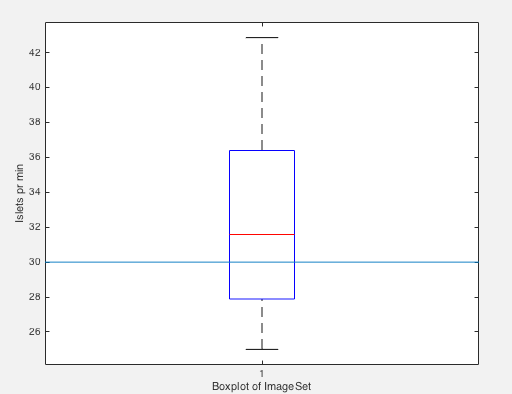
\includegraphics[width=0.5\textwidth]{billeder/software/boxplot.png}
	\caption{Boxplot af distrubutionen af øer pr. minut}
	\label{fig:boxplot}
\end{figure}

Selve flowsimuleringen sker i et for loop, hvor positionen for øen flyttes for hver iteration. I figur \ref{fig:flowsim} er flow simulationen illustreret for de i alt 18 sekvenser, med en graf for hver ø. Det ses at øen flytter sin Y position tilfældigt, mens X positionen springer med et fast interval for hver iteration i for loopet.

\begin{figure}[H]
	\centering
	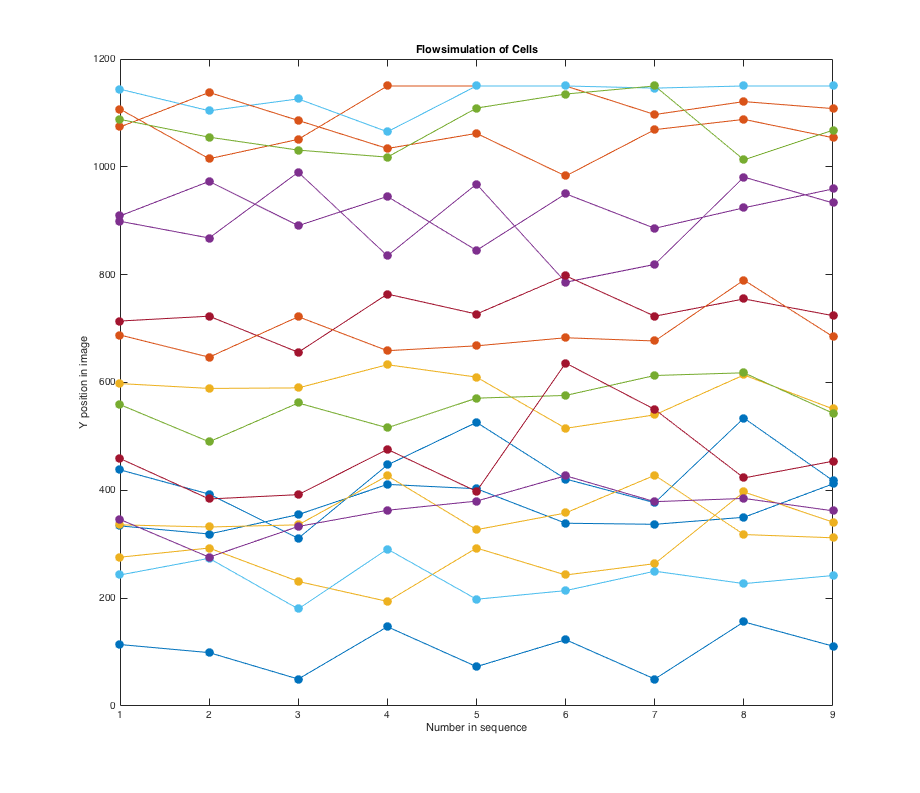
\includegraphics[width=0.5\textwidth]{billeder/software/Simulation.png}
	\caption{Illustration over flow simuleringen}
	\label{fig:flowsim}
\end{figure}


Øens position på billedet ændres ved en normalfordelt random variabel med mean på 0 og standard afvigelse på 50 pixels. Nedenstående figur \ref{fig:histfit} viser fordelingen af pixels øen flyttes for hver iteration. På figur \ref{fig:histfit} er der vist markører for standard afvigelsen ($\sigma$) og $2*$standard afvigelsen ($2\sigma$) for hver side af mean. I mellem $-\sigma$ og $\sigma$ er der 68,26 \% sandsynlighed for, at den nye Y position ville ligge inden for dette område. For 2 sd afvigelse ($2\sigma$) er der 95,45 \% for, at den nye Y position vil ligge inden for dette område.

\begin{figure}[H]
	\centering
	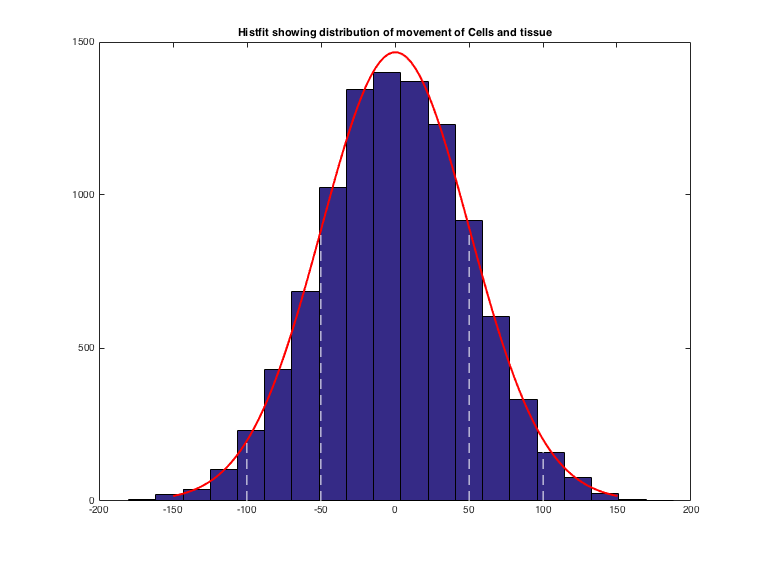
\includegraphics[width=0.5\textwidth]{billeder/software/histfit.png}
	\caption{Histogram over fordelingen af ny Y position}
	\label{fig:histfit}
\end{figure}

Det endelige resultat af billedegeneringen er vist i figur \ref{fig:finalresult}. Til at illustrere hvordan øen flytter sig er der tilføjet en graf, som viser hvordan dens position ændres for hver iteration. Øen er markeret med en rød ring på billedet.

\begin{figure}[H]
	\centering
	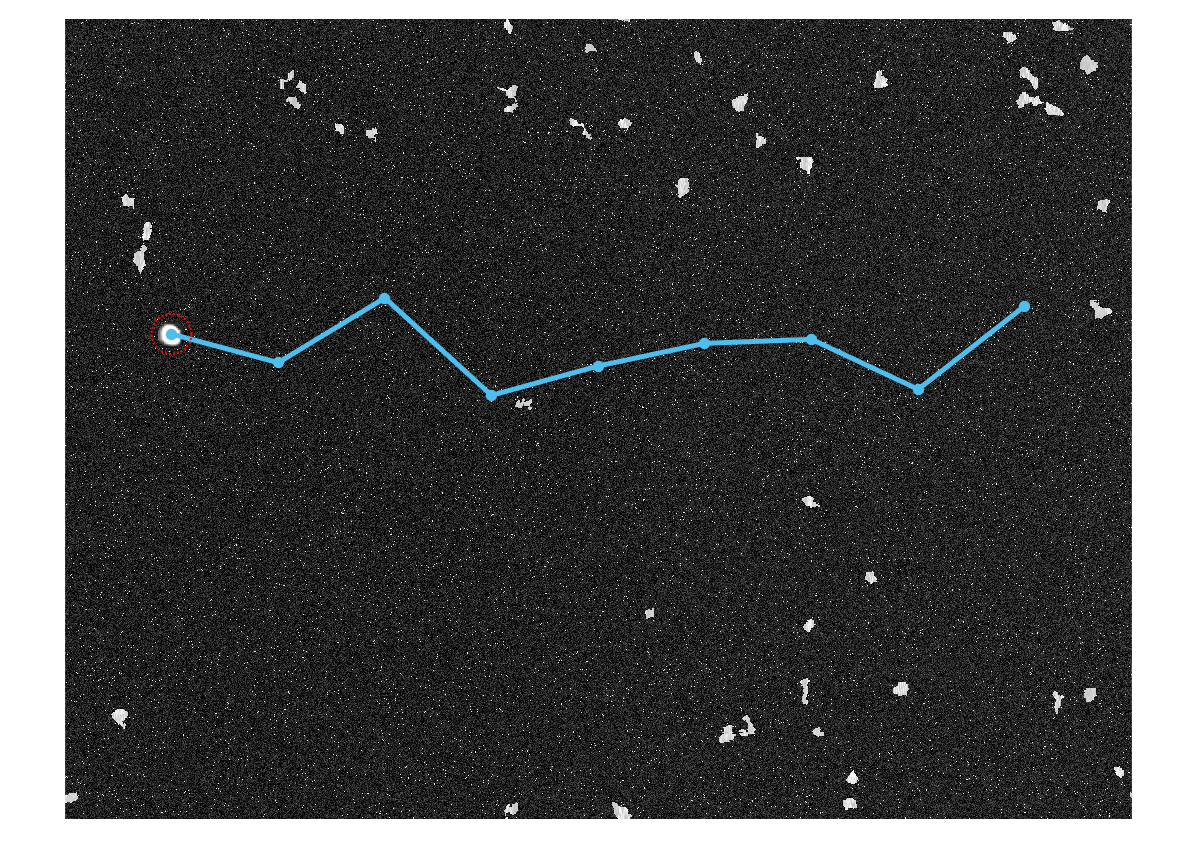
\includegraphics[width=0.7\textwidth]{billeder/software/final.png}
	\caption{Endelige resultat for flowsimulering}
	\label{fig:finalresult}
\end{figure}

\subsection{Billedprocessering}
Selve segmenteringen sker via en række morfologiske operationer, hvor billedet fra kamera simulationen konverteres til en logisk maske. Detektionenen baseres på, at øerne har en mere cirkulær form end resten af vævet. Derfor hentes der egenskaber fra objekterne i masken vha. matlab funktionen \textit{regionsprops}. De egenskaber der hentes er med til, at beskrive hvor cirkulært objektet er. De egenskaber som hentes er arealet, center positionen, omkredsen og excentriciteten. Excentriciteten beskriver hvor langstrakt objektet er. Hvis excentriciteten er 0 er det en perfekt cirkel mens det vil være en langstrakt ellipse hvis værdien er 1.

Ud fra arealet og omkredsen af objekterne anvendes de 2 nedenstående formler til bestemmelse af 2 værdier for radiusen af objektet:
\begin{align}
Areal = R1^2*\pi => R1 = \sqrt{\frac{\text{Areal}}{\pi}}
\end{align}
\begin{align}
Omkreds = 2*R2*\pi => R2 = \frac{\text{Omkreds}}{2*\pi}
\end{align}

Udfra disse 2 radius værdier, vil det objekt, hvor der er mindst forskel i mellem de 2, være det objekt der er mest cirkulært. Til at illustrere dette er der i figur \ref{fig:circleelip} vist en cirkel og en ellipse begge med samme areal. Udfra \textit{regionsprops} og de 2 formler for radius kan der bestemmes 2 radiuser for henholdsvis cirklen og ellipsen. Forskellen bestemmes ved, at trække de 2 beregnede værdier fra hinanden. I udregningerne nedenfor er den første kolonne værdier for cirklen, mens den anden er for ellipsen. Som det ses er forskellen mindst ved cirklen, hvilket indikerer, at den er mest cirkulær.
  
\begin{lstlisting} 
r1 =  100.0017   99.9380

r2 =  99.7978  105.7890

rDif = 0.2039    5.8510
\end{lstlisting} 

\begin{figure}[H]
	\centering
	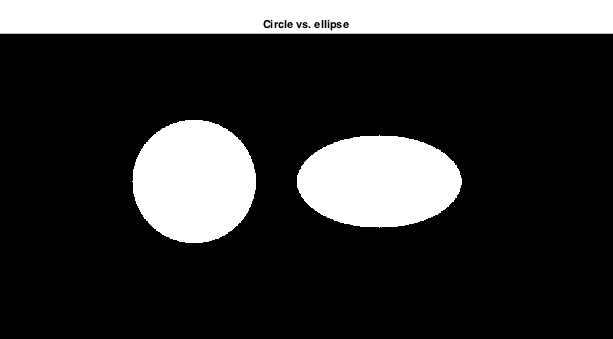
\includegraphics[width=0.6\textwidth]{billeder/software/circleellipse.png}
	\caption{Cirkel sammenlignet med ellipse}
	\label{fig:circleelip}
\end{figure}

Indekset for det objekt med mindst forskel i radius og indekset for det objekt med den mindste excentricitet gemmes i variabler. 
Til sidst i segmenteringen af den langerhanske ø kontrolleres det om radius forskellen og excentricitet ligger under nogle fast definerede grænseværdier. Værdierne er fundet ved, at analysere en række billeder og deres objekters radius og excentricitet. Radius og excentriciteten bliver gemt i logfilen, så de kan analyseres for senere at justere grænseværdierne. Hvis objektets værdier er under disse grænseværdier er en ø detekteret. Når en ø er detekteret illustreres det med en grøn ring på GUI.

For at løse udfordringen med, at den samme ø vil optræde på det næste billede, er der implementeret et smalt detekteringsvindue (100 pixels bredt). Når øen er detekteret inden for dette område bliver variablen isletDetected sat til true. Denne variabel anvendes til styring af ventilen. 
 
Figur \ref{fig:segmented} viser slutresultatet af segmenteringen, hvor masken kun indeholder den langerhanske ø fra det oprindelige billede. 


\begin{figure}[H]
	\centering
	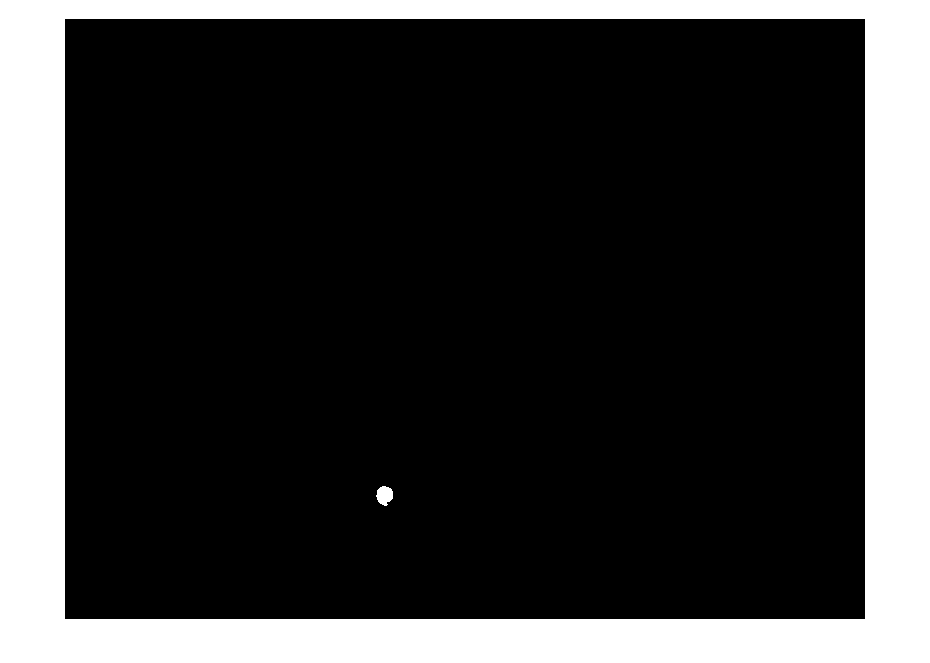
\includegraphics[width=0.6\textwidth]{billeder/software/segmented.png}
	\caption{Slutresultat af segmentering}
	\label{fig:segmented}
\end{figure}

I figur \ref{fig:finalimage} er det oprindelige billede vist, med markering af den detekterede ø.


\begin{figure}[H]
	\centering
	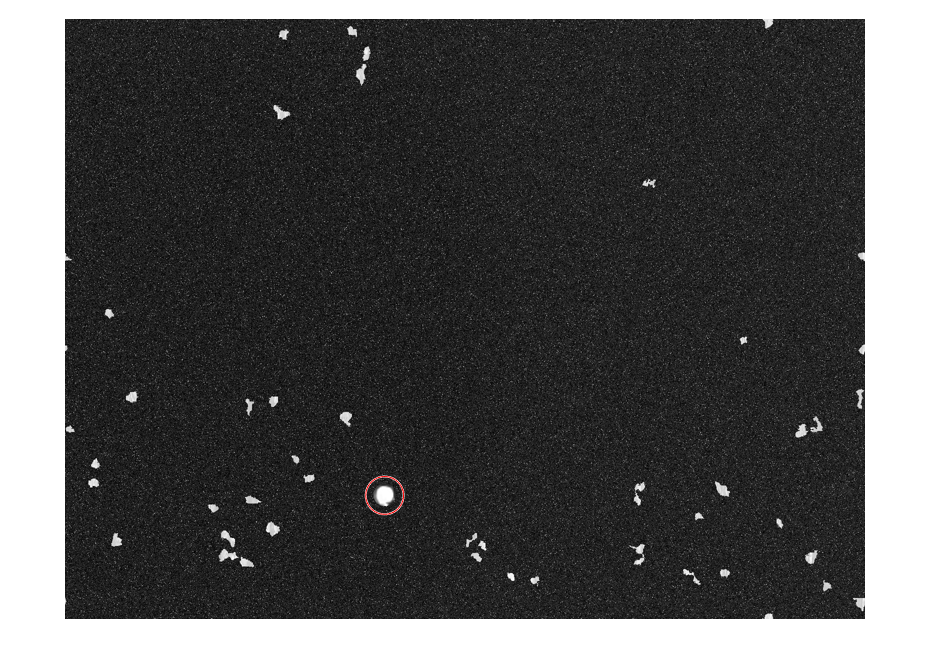
\includegraphics[width=0.6\textwidth]{billeder/software/finalimage.png}
	\caption{Oprindelige billede med detekteret ø}
	\label{fig:finalimage}
\end{figure}

\newpage
\textbf{Test af billedeprocessering}

En udfordring med billedeprocesseringen er, at hastigheden ikke må være for langsom i forhold til frameraten for kameraet. Da et nyt billede indlæses hvert 0,1 sekund skal billedprocesseringen dermed være hurtigere end dette for at følge med. Til test af dette er Matlab funktionen tic/toc anvendt, som måler hvor langt tid billedprocessingen tager om at eksekvere. I figur \ref{fig:dataprocess} viser grafen hvor lang tid det har taget, at behandle de enkelte billeder. Den røde streg viser den gennemsnitlige tid for processeringen. For den nuværende implementering tager billedeprocessingen 0,0104 sekund pr. billede, hvilket er indenfor grænsen på 0,1 sekund. Tiden vil variere alt efter tilgængelig processorkraft og om der skal udføres andre opgaver, eksempelvis opdatere figurer på GUI. 

\begin{figure}[H]
	\centering
	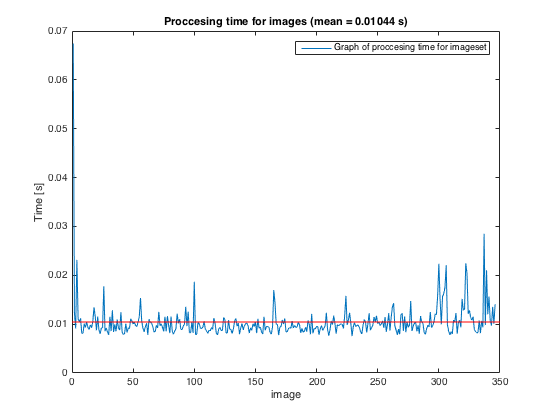
\includegraphics[width=0.6\textwidth]{billeder/software/dataprocessing_2.png}
	\caption{Test af tidsforbrug for billedeprocessering}
	\label{fig:dataprocess}
\end{figure}

\section{Simuleringsvæske}
\label{sec:simuleringsv}
Da de langerhanske øer ikke er lettilgængelig, har det været nødsaget at finde et objekt til at agere aktør for cellerne. Simuleringsvæsken skal bruges til at teste de mekaniske dele, samt tidsintervallet mellem kameraet og ventilen. Egenskaberne af de langerhanske øer der er brugt til at finde simuleringsvæsken er at de er runde og lyse, størrelsen, samt at de bundfælder i colleganse opløsningen. Der har været to iterationer for at finde en aktør for cellerne, den første har bestået i at finde perfekte runde og hvide objekter med en $massefylde<1$. Til dette blev der brugt polysterene, som er lettilgængelig, samt runde, hvide og kan fåes med en massefylde lige over en \fxnote{reference til bedre side end wiki?}. Dog blev det fundet svært at finde polysterene kugler i størrelsen 0.1-0.3mm, derfor blev der skabt kontakt til forhandlere af flamingo kugler. Dog var de tilsendte kugler for store, samt flød oven på. 

Den anden iteration bestod i at finde et biologisk materiale, hvor ved faktorerne runde og hvide blev nedprioriteret for at finde et objekt. For at finde en celle aktør med lettilgængelighed blev plantefrø den næste mulighed. Trods begrænset data omkring plantefrø, lykkes det gruppen at finde plantefrø i størrelsen 0.1-0.3mm vha. forhandlere af plantefrø og andre eksperter \fxnote{referencer til mail}. De indkøbte frø består af timian frø og rævehale frø \fxnote{indsæt billeder}. Udover de indkøbte frø kan der ved videre bearbejdelse af projektet overvejes transparent testa (tt4 mutant) frø. De skulle i følge \textit{Carsten Meier} være hvide, forholdsvis runde, dog er de ikke lige så tilgængelige, som de allerede indkøbte frø. Dette har været grunden til, at de ikke er brugt i projektet ind til nu. Derfor består den anvendte simuleringsvæske af, demineraliseret vand og timian plantefrø som aktør for de langerhanske øer.  
 
\section{Aceepttest af produktet} 
Til sidst i udviklingsforløbet blev der udført en accepttest af systemet. Den udførte accepttest er vedlagt i bilag XX. En række af kvalitetskravene blev ikke testet grundet kameraet ikke blev implementeret i prototypen. For hvert af kravene der ikke blev godkendt er der udfyldt en fejlrapport, hvor en handlingsplan beskriver hvordan og hvornår fejlen rettes. De udfyldte fejlrapporter er ligeledes vedlagt i bilag \ref{Fejlrapport}.

\newpage
\section{Cost-benefit analyse}
Dette afsnit indeholder cost-benefit analysen, som belyser hvilke omkostninger der er forbundet med sortering af langerhanske øer. Analysen sammenligner omkostningerne forbundet med den manuelle sorteringsproces og den automatiserede metode. Formålet med analysen er, at beregne hvad stk. prisen pr. ø er ved henholdsvis den ene og den anden metode. Dette anvendes til at give en tidshorisont for hvornår en investering af den automatiserede løsning vil være tjent hjem igen. Udgangspunktet for analysen bygger på det tidsmæssige forbrug der er forbundet med isolering af et batch på 400 øer fra mus. 

Fælles for begge sorteringsmetoder er, at der fortsat foretages manuel perfusion og nedbrydning og vaskning af pankreas. Nedenstående tabel opsummere hvilke basisudgifter der er forbundet ved disse processer. Timelønnen er beregnet ud fra en PhD studerendes månedsløn på 25.040 kr \citep{phdwage}.
\begin{center}
		\begin{longtable}{ | m{6cm} | m{1.5cm} | m{1.5cm} | m{3cm}| } 
			\hline
			 &\textbf{Antal} & \textbf{Pris} & \textbf{Total}\\ 
			\hline
			 \textbf{Mus} & 6 stk & 60 kr & 360 kr\\ 
			\hline
			 \textbf{Tid for perfusion} & 1 time & 171,62 kr & 171,62 kr\\ 
			\hline
			\textbf{Tid for nedbrydning + vask} & 1 time & 171,62 kr & 171,62 kr\\ 
			\hline	
			\textbf{Total} &  &  & \textbf{703,24 kr}\\ 
			\hline
			\caption{Basis omkostninger for sorteringsproces}
			 		\end{longtable}
\end{center}
Nedenstående tabel \ref{tab:sortcost} viser, hvilke omkostninger der er forbundet med selve isoleringsprocessen af de langerhanske øer. Den halve time der bruges ved den automatiske metode er et estimat af hvad der skal bruges på påfyldning af beholdere og start af sorteringsproces. 
\begin{center}
		\begin{longtable}{ | m{6cm} | m{1.5cm} | m{1.5cm} | m{3cm}| } 
			\hline
			 &\textbf{Antal} & \textbf{Pris} & \textbf{Total}\\ 
			\hline
			 \textbf{Tid manuel} & 6 timer & 171,62 kr & 1029,73 kr\\ 
			\hline
			 \textbf{Tid automatisk} & 0,5 timer & 171,62 kr & 85,81 kr\\ 
			\hline
			\caption{Omkostninger ved sortering af langerhanske øer}
			\label{tab:sortcost}
			 		\end{longtable}
\end{center}
Omkostningerne ved de to sorteringsmetoder er opsummeret i tabel \ref{tab:totalcost}, herunder en samlet pris for et batch på 400 øer, og en stk. pris pr. ø for hver sorteringsmetode.
\begin{center}
		\begin{longtable}{ | m{8cm} | m{2.25cm} | m{2.25cm} | } 
			\hline
			 &\textbf{Manuelt} & \textbf{Automatisk} \\ 
			\hline
			 \textbf{Basis omkostninger} & 703,24 kr & 703,24 kr \\ 
			\hline
			 \textbf{Isoleringsomkostninger} & 1029,73 kr & 85,81 kr \\ 
			\hline
			\textbf{Total pris for sortering} & 1732,97 kr & 789,05 kr \\ 
			\hline
			\textbf{Pris pr. ø ved batch på 400 stk} & 4,33 kr & 1,97 kr \\ 
			\hline
			\caption{Opsummering af omkostninger for sorteringsprocesen for de to sorteringsmetoder}
			\label{tab:totalcost}
			 		\end{longtable}
\end{center}

Da der er forbundet omkostninger ved en investering i et system til automatisk isolering, er udgifterne til den udviklede prototype opsummeret i tabel \ref{tab:prototypecost}. I tabellen er de enkelte hardware komponenters pris noteret, samt hvad en licens til Matlab koster. Herudover er der vurderet en profit på 400 \% af udgifterne til hardware komponenter og Matlab licens. Denne udgift dækker udgifter til support og vedligehold, produktion, monteringsomkostninger, garanti og udvikling. Som det ses i tabellen er udgiften til den udviklede prototype beregnet til 86175 kr.
\begin{center}
		\begin{longtable}{ | m{9.5cm} | m{3.5cm} | } 
			\hline
			  & \textbf{Pris} \\ 
			\hline
			Kamera & 400 kr \\ 
			\hline
			 Ventil & 845 kr\\ 
			\hline
			Pumpe & 80 kr  \\ 
			\hline
			Arduino & 150 kr \\ 
			\hline
			Andet hardware & 210 kr \\ 
			\hline
			Beholdere + slanger & 425 kr \\ 
			\hline
			3d print & 125 kr \\ 
			\hline
			Matlab licens & 15000 kr \\
			\hline
			Profit på 400\% & 68940 kr \\	
			\hline
			\textbf{Total pris} & \textbf{86175 kr} \\		
			
			\hline
			\caption{Udgifter til automatiseret system}
			\label{tab:prototypecost}
			 		\end{longtable}
\end{center}


\newpage
Til at illustrere og sammenligne udgifterne for de to sorteringsmetoder viser figur \ref{fig:costbenefit} udgiften over tid. Figuren viser omkostningerne set over en periode på 2 år, ved at der sorteres et batch pr. uge.

\begin{figure}[H]
	\centering
	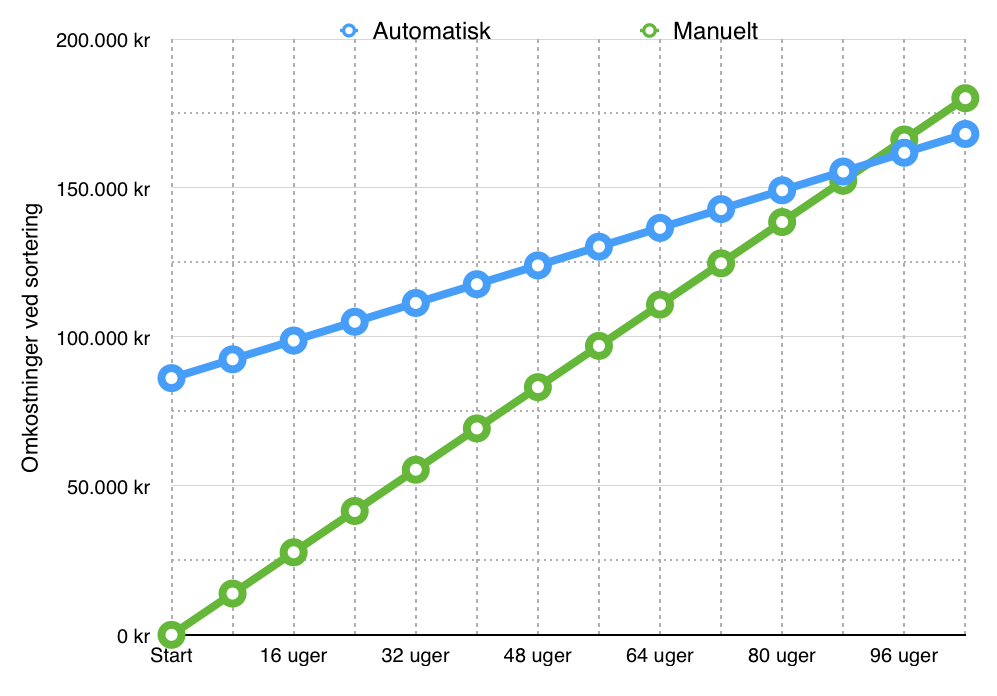
\includegraphics[width=1\textwidth]{billeder/Hovedrapport/costbenefit2.png}
	\caption{Udvikling i omkostninger }
	\label{fig:costbenefit}
\end{figure}

Af figur \ref{fig:costbenefit} ses det, at efter 92 uger overstiger omkostningerne ved den manuelle sorteringsproces de omkostninger der er ved den automatiske, og investeringen vil her være tjent hjem. 